\chapter{Results}
\label{ch:results}


\begin{figure}[hbt!]
 %\centering
 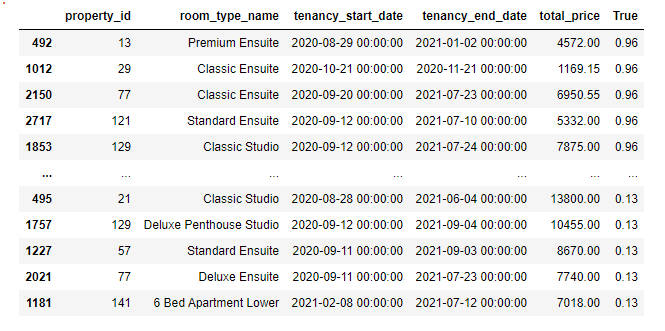
\includegraphics[width=15cm]{figures/canc_prob.png}
 \caption{Predictions made on the test dataset, ranking bookings by percentage chance cancelled. This is what will be added into the booking management system to help understand what bookings will be cancelled}
\end{figure}

\section{XGboost}

for the section I run the algorithm manually so I could evaluate a comparison of the results between the automated ml model and using the standard XGboost library with no \textbf{hyper parameter tuning or feature stuff}


\begin{figure}[hbt!]
 %\centering
 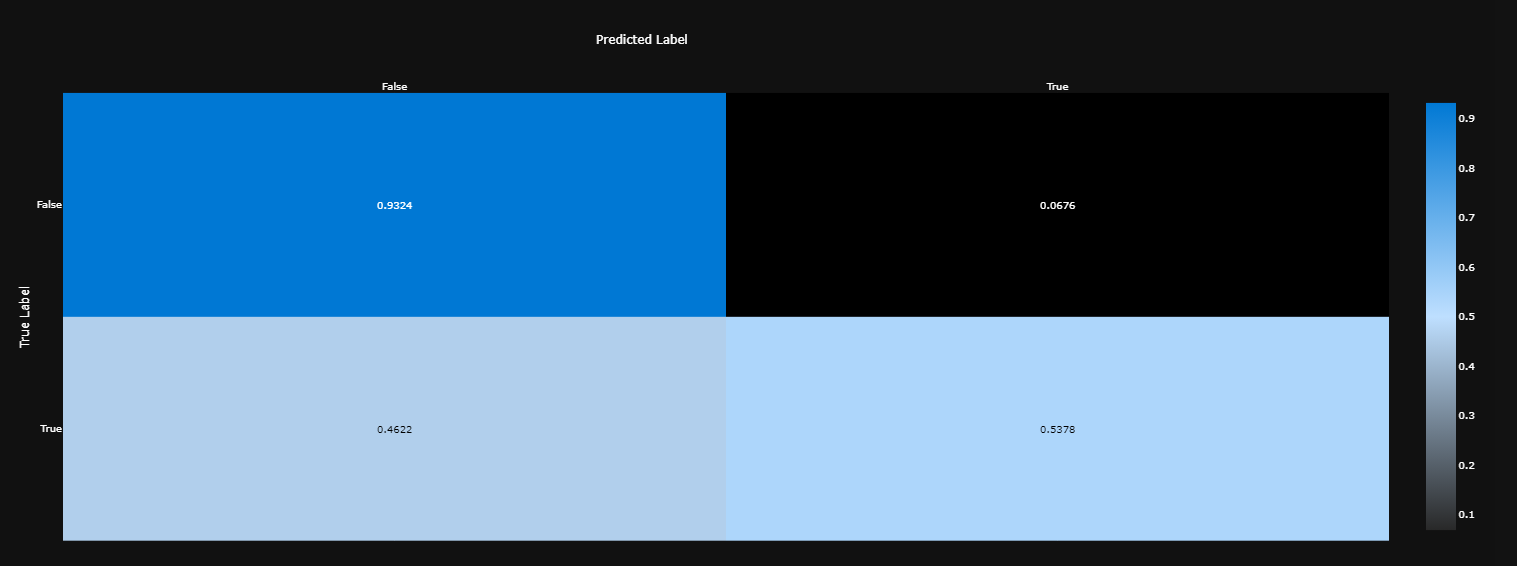
\includegraphics[width=15cm]{figures/azure_ml_confusion_matrix_xg.png}
 \caption{The confusion matrix output from the XGBoost algorithm shows a close to 50-50 slit when comparing Actual True with false positive. This shows bad \textbf{recall?}}
\end{figure}


\section{Auto ML}

Here I used Auto ML to evaluate and compare \textbf{some number} of different algorithms looking at the norm macro recall as the target value instead of the accuracy as this reduces false positive rate

\begin{figure}[hbt!]
 %\centering
 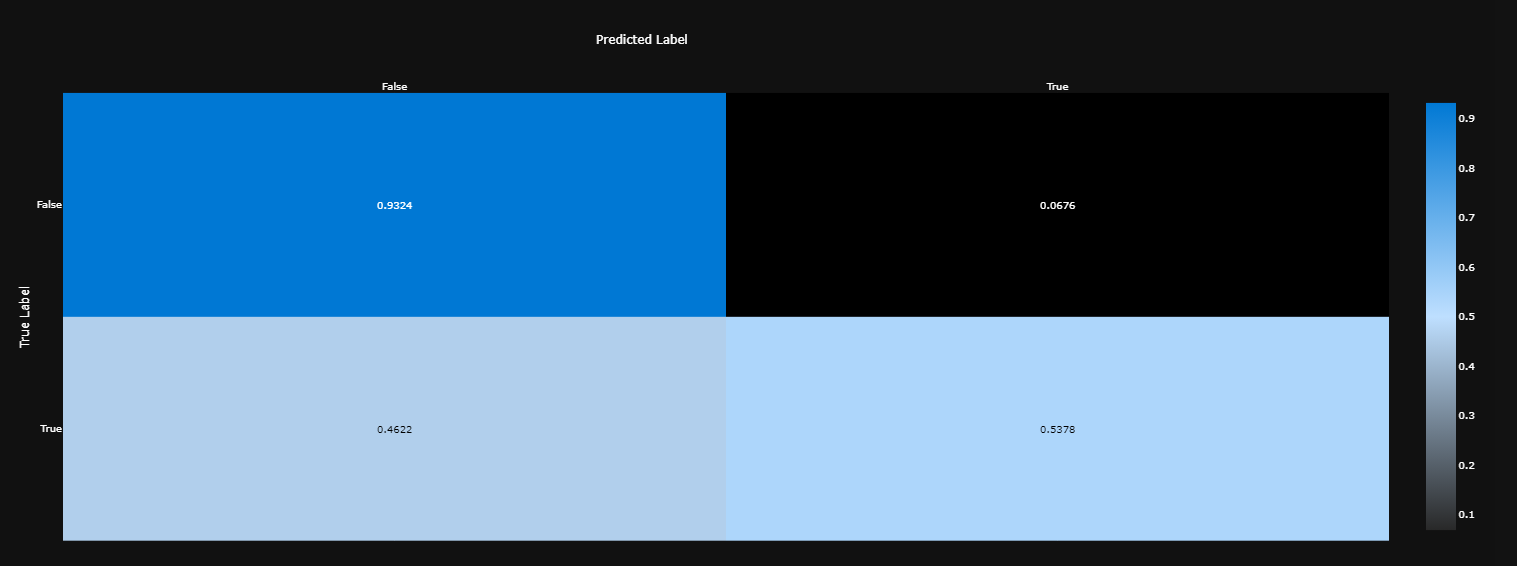
\includegraphics[width=15cm]{figures/azure_ml_confusion_matrix_xg.png}
 \caption{The confusion matrix output from the XGBoost algorithm shows a close to 50-50 slit when comparing Actual True with false positive. This shows bad \textbf{recall?}}
\end{figure}